% !TeX program = pdflatex
% !BIB program = bibtex
% Template LaTeX file for DAFx-19 papers
%
% To generate the correct references using BibTeX, run
%     latex, bibtex, latex, latex
% modified...
% - from DAFx-00 to DAFx-02 by Florian Keiler, 2002-07-08
% - from DAFx-02 to DAFx-03 by Gianpaolo Evangelista
% - from DAFx-05 to DAFx-06 by Vincent Verfaille, 2006-02-05
% - from DAFx-06 to DAFx-07 by Vincent Verfaille, 2007-01-05
%                          and Sylvain Marchand, 2007-01-31
% - from DAFx-07 to DAFx-08 by Henri Penttinen, 2007-12-12
%                          and Jyri Pakarinen 2008-01-28
% - from DAFx-08 to DAFx-09 by Giorgio Prandi, Fabio Antonacci 2008-10-03
% - from DAFx-09 to DAFx-10 by Hannes Pomberger 2010-02-01
% - from DAFx-10 to DAFx-12 by Jez Wells 2011
% - from DAFx-12 to DAFx-14 by Sascha Disch 2013
% - from DAFx-15 to DAFx-16 by Pavel Rajmic 2015
% - from DAFx-16 to DAFx-17 by Brian Hamilton 2016
% - from DAFx-18 to DAFx-19 by Dave Moffat 2019
%
% Template with hyper-references (links) active after conversion to pdf
% (with the distiller) or if compiled with pdflatex.
%
% 20060205: added package 'hypcap' to correct hyperlinks to figures and tables
%                      use of \papertitle and \paperauthorA, etc for same title in PDF and Metadata
%
% 1) Please compile using latex or pdflatex.
% 2) If using pdflatex, you need your figures in a file format other than eps! e.g. png or jpg is working
% 3) Please use "paperftitle" and "pdfauthor" definitions below

%------------------------------------------------------------------------------------------
%  !  !  !  !  !  !  !  !  !  !  !  ! user defined variables  !  !  !  !  !  !  !  !  !  !  !  !  !  !
% Please use these commands to define title and author(s) of the paper:
\def\papertitle{Stable Structures for Nonlinear Biquad Filters}
\def\paperauthorA{Jatin Chowdhury}

% Authors' affiliations have to be set below

%------------------------------------------------------------------------------------------
\documentclass[twoside,a4paper]{article}
\usepackage{dafx_19}
\usepackage{amsmath,amssymb,amsfonts,amsthm}
\usepackage{euscript}
\usepackage[latin1]{inputenc}
\usepackage[T1]{fontenc}
\usepackage{ifpdf}

\usepackage[english]{babel}
\usepackage{caption}
\usepackage{subfig} % or can use subcaption package
\usepackage{xcolor}

\setcounter{page}{1}
\ninept

\usepackage{times}
% Saves a lot of ouptut space in PDF... after conversion with the distiller
% Delete if you cannot get PS fonts working on your system.

% pdf-tex settings: detect automatically if run by latex or pdflatex
\newif\ifpdf
\ifx\pdfoutput\relax
\else
   \ifcase\pdfoutput
      \pdffalse
   \else
      \pdftrue
\fi

\ifpdf % compiling with pdflatex
  \usepackage[pdftex,
    pdftitle={\papertitle},
    pdfauthor={\paperauthorA},
    colorlinks=false, % links are activated as colror boxes instead of color text
    bookmarksnumbered, % use section numbers with bookmarks
    pdfstartview=XYZ % start with zoom=100% instead of full screen; especially useful if working with a big screen :-)
  ]{hyperref}
  \pdfcompresslevel=9
  \usepackage[pdftex]{graphicx}
  \usepackage[figure,table]{hypcap}
\else % compiling with latex
  \usepackage[dvips]{epsfig,graphicx}
  \usepackage[dvips,
    colorlinks=false, % no color links
    bookmarksnumbered, % use section numbers with bookmarks
    pdfstartview=XYZ % start with zoom=100% instead of full screen
  ]{hyperref}
  % hyperrefs are active in the pdf file after conversion
  \usepackage[figure,table]{hypcap}
\fi

% My packages
\usepackage{cleveref}
\usepackage{tikz}
\usetikzlibrary{dsp,chains}
\usepackage{tkz-euclide}
\usetkzobj{all}

\usepackage{listings}
\definecolor{codegreen}{rgb}{0,0.6,0}
\definecolor{codegray}{rgb}{0.5,0.5,0.5}
\definecolor{codepurple}{rgb}{0.58,0,0.82}
\definecolor{backcolour}{rgb}{0.95,0.95,0.92}
 
\lstdefinestyle{mystyle}{
    backgroundcolor=\color{backcolour},   
    commentstyle=\color{codegreen},
    keywordstyle=\color{magenta},
    numberstyle=\tiny\color{codegray},
    stringstyle=\color{codepurple},
    basicstyle=\footnotesize,
    columns=flexible,
    breakatwhitespace=false,         
    breaklines=true,                 
    captionpos=b,                    
    keepspaces=true,                               
    showspaces=false,                
    showstringspaces=false,
    showtabs=false,                  
    tabsize=4
}
 
\lstset{style=mystyle}

\DeclareMathAlphabet{\mathpzc}{OT1}{pzc}{m}{it}
\newcommand{\z}{\mathpzc{z}}

\title{\papertitle}

\affiliation{
\paperauthorA \,}
{\href{http://ccrma.stanford.edu}{Center for Computer Research in Music and Acoustics} \\ Stanford University \\ Palo Alto, CA \\ {\tt \href{mailto:jatin@ccrma.stanford.edu}{jatin@ccrma.stanford.edu}}}

\begin{document}
% more pdf-tex settings:
\ifpdf % used graphic file format for pdflatex
  \DeclareGraphicsExtensions{.png,.jpg,.pdf}
\else  % used graphic file format for latex
  \DeclareGraphicsExtensions{.eps}
\fi

\maketitle

\begin{abstract}
Biquad filters are a common tool for filter design. In this
writing, we develop two structures for creating biquad filters
with nonlinear elements. We derive expressions for the instantaneous pole
locations of each nonlinear filter, and provide conditions for
their guaranteed stability. Finally, we examine example filters
built with these nonlinear structures, and show how the first
nonlinear structure can be used in the context of analog modelling.
\end{abstract}

\section{Introduction}
A ``biquad'' filter refers to a general 2nd order IIR filter.
In digital signal processing, biquad filters are often useful
since any higher-order filter can be implemented using a cascade
of biquad filters. While digital biquad filters are typically implemented
as linear processors, for audio applications it can be useful to
implement nonlinear filters. For example, in \cite{SKF} the authors
use a passive model of operational amplifiers to model the nonlinear
behaviour of a Sallen-Key lowpass filter. Meanwhile, in \cite{Vadim},
the author proposes several methods for using nonlinear elements
to enhance linear models of analog ladder filters. More relevant to
our current topic is \cite{Rossum1992MakingDF}, in which the author
suggests a method for altering a general digital feedback filter
by saturating the feedback path, with the goal of achieving a more
analog-like response. In this writing, we strive
to develop more general nonlinear filter structures. While these structures
may be used for analog modelling, they do not necessarily depend on analog
modelling principles to be understood and implemented.

\section{Structural Elements}
\subsection{Linear Filter}
%
We begin with the equation for a biquad filter:
%
\begin{equation}
\begin{split}
    y[n] = b_0 u[n] + b_1 u[n-1] + b_2 u[n-2] \\ - a_1 y[n-1] - a_2 y[n-2]
\end{split}
    \label{eq:bq}
\end{equation}
%
Where $y$ is the output signal, $u$ is the input signal, and $a_n$ and $b_n$
are the feed-back and feed-forward filter coefficients, respectively.
There are several convenient "direct forms" for implementing biquad filters.
In this writing we will focus on the ``Transposed Direct Form II'' (TDF-II),
which is popular for its numerical properties \cite{JOSFilters}.
%
\begin{figure}[ht]
    \center
    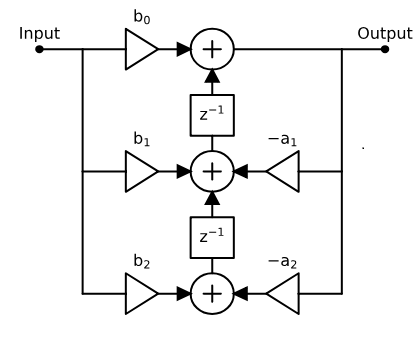
\includegraphics[width=2.3in]{../Pics/TDF-II-White.png}
    \caption{\label{TDF-II}{\it Transposed Direct Form II}}
\end{figure}
%
Note that the poles of the filter can be described using the quadratic
equation.
\begin{equation}
    p = \frac{-a_1 \pm \sqrt{a_1^2- 4a_2}}{2}
    \label{eq:poles_lin}
\end{equation}
%
Specifically, the pole magnitude is equal to:
\begin{equation}
    |p|^2 = \frac{-a_1 + \sqrt{a_1^2- 4a_2}}{2} \frac{-a_1 - \sqrt{a_1^2- 4a_2}}{2} = |a_2|
    \label{eq:poles_lin_mag}
\end{equation}
%
And the angular frequencies of the poles are equal to
(assuming complex poles):
\begin{equation}
    \angle p = \arctan \left(\pm \frac{\sqrt{|a_1^2- 4a_2|}}{a_1} \right)
    \label{eq:poles_lin_angle}
\end{equation}
%
It is well known that a digital filter will be stable provided that
the magnitudes of the poles are strictly less 1 \cite{JOSFilters}.

\subsection{Nonlinear Elements}
%
We now propose adding nonlinear elements to the above filter structure.
We will refer to these nonlinear elements as ``base nonlinearities''
To keep the discussion as broad as possible, we consider any one-to-one
nonlinear function $f_{NL}(x)$.
\newline\newline
In analog modelling literature, it is
common to "linearize" a nonlinear function around a certain operating
point. This process is typically done by constructing a Thevenin or
Norton equivalent circuit that represents the nonlinear function at
that operating point, where the resistance of the equivalent circuit
is determined by the slope of the nonlinearity at the operating point,
and the source of the equivalent circuit is determined by the DC
offset of the linearized system at the operating point
\cite{BernersDAFX}.
\newline\newline
In our purely digital formulation, we can linearize a nonlinear function
as a gain element plus a constant source (see \cref{linize}).
%
\begin{figure}[!ht]
    \center
    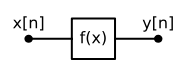
\includegraphics[width=1.0in]{../Pics/NL_sys_trim_white.png}
    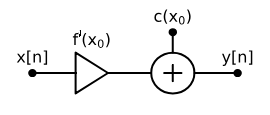
\includegraphics[width=1.4in]{../Pics/NL_sys_lin_white.png}
    \caption{\label{linize}{\it A general digital nonlinear system (left),
                                and a general linearization of that system (right).}}
\end{figure}
%
For operating point $x_0$:
%
\begin{equation}
    \bar{f}_{NL}(x) = f'_{NL}(x_0)x + c(x_0)
    \label{eq:linearized}
\end{equation}
%
where the offset $c(x_0)$ is described by
%
\begin{equation}
    c(x_0) = f_{NL}(x_0) - f'_{NL}(x_0)x_0
    \label{eq:lin_off}
\end{equation}
%
In \cref{tanh_lin}, we show an example of linearizing the nonlinear
function $f_{NL}(x) = \tanh(x)$ at $x_0=1$.
%
\begin{figure}[h]
    \center
    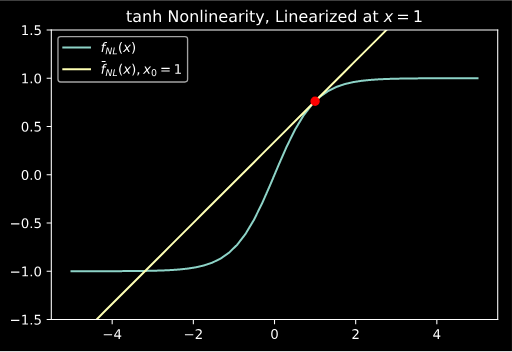
\includegraphics[width=3in]{../Pics/tanh_linized.png}
    \caption{\label{tanh_lin}{\it $\tanh$ nonlinearity, linearized at $x=1$.}}
\end{figure}
%
\subsubsection{Stability Constraints}

In order to guarantee that the filters we construct in the next section
will be stable, we propose the following constraint on the base
nonlinearities used to construct nonlinear filters:
%
\begin{equation}
    0 \leq f'_{NL}(x) \leq 1
    \label{eq:NL_constraint}
\end{equation}
%
In other words, the nonlinearities must be monotonic and may never have
a slope greater than 1. Many typical musical nonlinearities satisfy
this constraint, including saturating, dropout, and half-wave rectifying
nonlinearities. Of particular interest to us will be saturating
nonlinearities, including hard-clippers, soft-clippers, and sigmoid-like
functions (see \cref{Sats}).
Saturating nonlinearities satisfy the property that
%
\begin{equation}
    |x| \rightarrow \infty, \ f'_{sat}(x) \rightarrow 0
    \label{eq:Sat_constraint}
\end{equation}
%
\begin{figure}[h]
    \center
    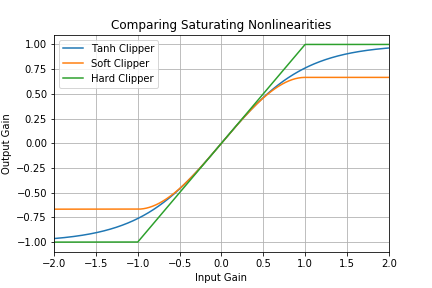
\includegraphics[width=3in]{../Pics/Sat-NLs.png}
    \caption{\label{Sats}{\it Saturating Nonlinearities}}
\end{figure}
%

\section{Nonlinear Filter Structure 1: Nonlinear Biquad}
%
\begin{figure*}[ht]
    % \center
    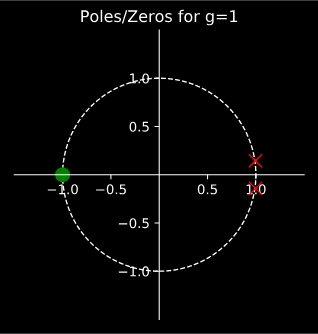
\includegraphics[width=1.7in]{../Pics/pz1.png}
    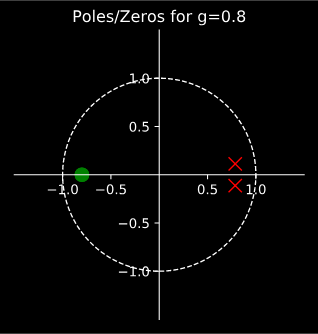
\includegraphics[width=1.7in]{../Pics/pz08.png}
    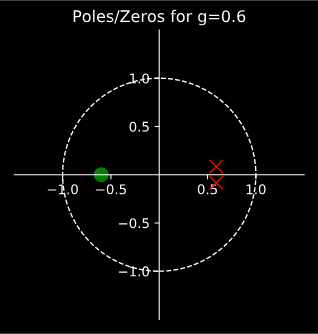
\includegraphics[width=1.7in]{../Pics/pz06.png}
    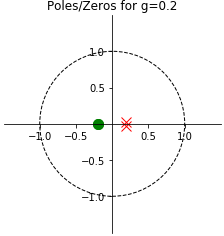
\includegraphics[width=1.7in]{../Pics/pz02.png}
    \caption{\label{pzPlots}{\it Instantaneous poles for a nonlinear biquad resonant
                                lowpass filter at varying input levels.}}
\end{figure*}
%
\begin{figure}[ht]
    \center
    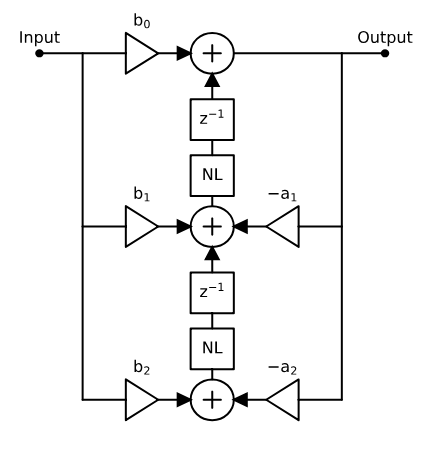
\includegraphics[width=2.3in]{../Pics/NL-TDF-II-White.png}
    \caption{\label{NL-TDF-II}{\it Nonlinear Transposed Direct Form II.
                                The ``NL'' blocks refer to a generalized
                                nonlinear element.}}
\end{figure}
%
We now propose adding nonlinear elements to the TDF-II strcuture in the
following fashion (see \cref{NL-TDF-II}). We will refer to this structure
as the ``Nonlinear Biquad''.
%
The equation for the nonlinear biquad filter then becomes:
%
\begin{equation}
\begin{split}
    y[n] = b_0 u[n]
         + f_{NL} (b_1 u[n-1] - a_1 y[n-1] \\
         + f_{NL} (b_2 u[n-2] - a_2 y[n-2]))
\end{split}
    \label{eq:bq_NL}
\end{equation}
%
Here it can be useful to define filter ``state variables''
as the inputs to the nonlinearities.
%
\begin{equation}
\begin{split}
    x_1 &= f_{NL} (x_2) + b_1 u[n-1] - a_1 y[n-1] \\
    x_2 &= b_2 u[n-2] - a_2 y[n-2]
\end{split}
    \label{eq:states}
\end{equation}
%
Note that for saturating base nonlinearities, as the input $u$ grows large,
the other terms will become negigible.
\newline\newline
Now we can replace the nonlinear elements with their linearized
models, using the state variables to define the operating points.
To make our notation more concise, we will denote the
output of the nonlinear functions as follows:
\begin{equation}
\begin{split}
    & \bar{f}_{NL_k}(x) = g_k x + \gamma_k \\
    & g_k = f'_{NL}(x_k), \; \gamma_k = c(x_k)
\end{split}
    \label{eq:linearized_bqnls}
\end{equation}
Then \cref{eq:bq_NL} can be re-written:
%
\begin{equation}
\begin{split}
    y[n] = b_0 u[n]
         + g_1 (b_1 u[n-1] - a_1 y[n-1] \\
         + g_2 (b_2 u[n-2] - a_2 y[n-2]) + \gamma_2) + \gamma_1
\end{split}
    \label{eq:bq_re-write}
\end{equation}
%
Finally, we can re-write the filter coefficients as variables dependent on
the state variables:
%
\begin{align}
\begin{split}
    b_0' &= b_0\\
    b_1' &= g_1 b_1\\
    b_2' &= g_1g_2 b_2\\
    a_1' &= g_1 a_1\\
    a_2' &= g_1g_2 a_2
\end{split}
    \label{eq:bq_coefs_re-write}
\end{align}
%
\begin{equation}
\begin{split}
    y'[n] &= b_0' u[n]
    + b_1' u[n-1] - a_1' y[n-1] \\
    & + b_2' u[n-2] - a_2' y[n-2]
    + g_1\gamma_2 + \gamma_1
\end{split}
    \label{eq:bq_re-write2}
\end{equation}
%
Note that the two $\gamma$ terms in \cref{eq:bq_re-write2} are simple
offsets as defined by our linearized model, and as such will not
affect the pole locations, nor the filter stability.

\subsection{Guaranteed Stability}
%
Since the coefficients of the biquad filter will be dependent on the
state of the filter, the instantaneous poles of the filter will be
dependent as well. In order to calculate the instantaneous poles of
the nonlinear biquad structure, we can adjust the formula from
\cref{eq:poles_lin}.
%
\begin{equation}
    p' = \frac{-g_1 a_1 \pm \sqrt{g_l^2 a_1^2- 4 g_1 g_2 a_2}}{2}
    \label{eq:poles_nl}
\end{equation}
%
From the constraint in \cref{eq:NL_constraint}, we can see that the
magnitude of the instantaneous pole will always be less than or equal to
the magnitude of the original pole from the corresponding linear filter.
Therefore, we know that any nonlinear biquad filter designed with the above
structure will be stable provided that the corresponding linear filter is
stable, and that the constraint from \cref{eq:NL_constraint} is satisfied.
\newline\newline
For saturating base nonlinearities, we can see from \cref{eq:Sat_constraint}
that as the state variables grow large, the poles will go to zero.
\newline\newline
The pole magnitude and angle with move as follows.
\begin{equation}
    |p'|^2 = \frac{g_1^2 a_1^2 - (g_l^2 a_1^2- 4 g_1 g_2 a_2)}{4} = g_1 g_2 a_2 = g_1 g_2 |p|^2
    \label{eq:poles_nl_mag}
\end{equation}
%
\begin{equation}
\begin{split}
    \angle p' = \arctan \left(\pm \frac{\sqrt{|g_1^2 a_1^2- 4g_1g_2a_2|}}{g_1a_1} \right) \\
    = \arctan \left(\pm \frac{\sqrt{\left|a_1^2- 4\frac{g_2}{g_1}a_2 \right|}}{a_1} \right)
\end{split}
    \label{eq:poles_nl_angle}
\end{equation}
%
Note that while the two gains are approximately the equal, the nonlinear
pole will have the same angle as the corresponding linear pole. An example
of this pole movement can be seen in \cref{pzPlots}.


\section{Nonlinear Filter Structure 2: Nonlinear Feedback Filter}
%
%
\begin{figure*}[!ht]
    % \center
    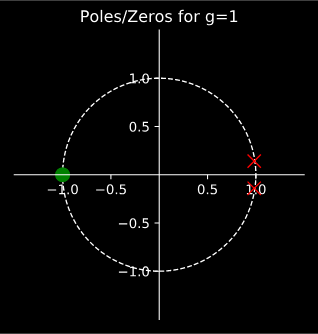
\includegraphics[width=1.7in]{../../NonlinearFeedback/Pics/pz1.png}
    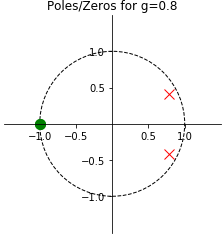
\includegraphics[width=1.7in]{../../NonlinearFeedback/Pics/pz08.png}
    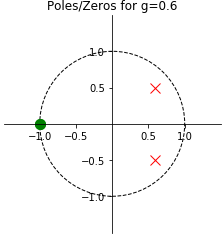
\includegraphics[width=1.7in]{../../NonlinearFeedback/Pics/pz06.png}
    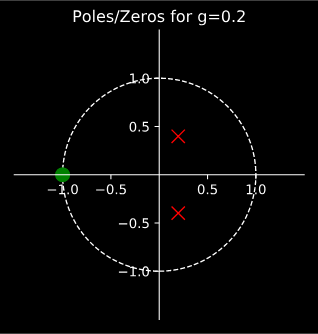
\includegraphics[width=1.7in]{../../NonlinearFeedback/Pics/pz02.png}
    \caption{\label{pzPlots2}{\it Instantaneous poles for a resonant
                                lowpass filter with nonlinear feedback
                                at varying input levels.}}
\end{figure*}
%
We now propose a different structure for adding elements to a TDF-II
Biquad filter, this time adding nonlinear elements to the feedback
paths (see \cref{NL2-TDF-II}). Note that though the two structures are developed
separately here, they could certainly be combined into a third structure,
which will also be stable under the same conditions as the two original
structures.
%
\begin{figure}[ht]
    \center
    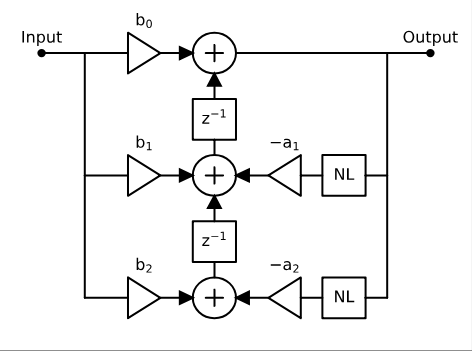
\includegraphics[width=2.3in]{../../NonlinearFeedback/Pics/NL2-TDF-II-White.png}
    \caption{\label{NL2-TDF-II}{\it Nonlinear Feedback Filter.}}
\end{figure}
%
The equaton for the filter can now be written:
%
\begin{equation}
    \begin{split}
        y[n] = b_0 u[n] + b_1 u[n-1] + b_2 u[n-2] \\ - a_1 f_{NL}(y[n-1]) - a_2 f_{NL}(y[n-2])
    \end{split}
        \label{eq:nlbq2}
\end{equation}
%
Again, we can replace the nonlinear elements with their linearized
models, this time using the $y[n-1]$ and $y[n-2]$ terms to define our
operating points.
%
\begin{equation}
    \begin{split}
        & \bar{f}_{NL_k}(x) = g_k x + \gamma_k \\
        & g_k = f'_{NL}(y[n-k]), \; \gamma_k = c(y[n-k])
    \end{split}
        \label{eq:gs2}
\end{equation}
%
And again, the filter equation can be re-written:
%
\begin{equation}
    \begin{split}
        y[n] & = b_0 u[n] + b_1 u[n-1] + b_2 u[n-2] \\
        & - a_1 (g_1 y[n-1] + \gamma_1)
        - a_2 (g_2 y[n-2] + \gamma_2)
    \end{split}
        \label{eq:nlbq2_rewrite}
\end{equation}
%
Or by re-writing the filter coefficients, we see:
%
\begin{align}
    \begin{split}
        b_0' &= b_0\\
        b_1' &= b_1\\
        b_2' &= b_2\\
        a_1' &= g_1 a_1\\
        a_2' &= g_2 a_2
    \end{split}
        \label{eq:bq2_coefs_re-write}
\end{align}
%
\begin{equation}
    \begin{split}
        y'[n] &= b_0' u[n]
        + b_1' u[n-1] - a_1' y[n-1] \\
        & + b_2' u[n-2] - a_2' y[n-2]
        - a_1\gamma_1 - a_2\gamma_2
    \end{split}
        \label{eq:nlbq2_re-write2}
\end{equation}
%
Again, the $\gamma$ offset terms will not affect the filter stability.

\subsection{Guaranteed Stability}
%
We can now calculate the locations of the instantaneous poles for
the nonlinear feedback filter, again by adjusting the formula from
\cref{eq:poles_lin}.
%
\begin{equation}
p' = \frac{-g_1 a_1 \pm \sqrt{g_1^2 a_1^2 - 4 g_2 a_2}}{2}
    \label{eq:poles_nl2}
\end{equation}
%
Again, we see that the nonlinear feedback filter will be stable, provided
that the corresponding linear filter is stable, and the constraint from
\cref{eq:NL_constraint} is satisfied.
\newline\newline
In this case the pole magnitude and angle will move as follows:
\begin{equation}
    |p'|^2 = \frac{g_1^2 a_1^2 - (g_l^2 a_1^2- 4 g_2 a_2)}{4} = g_2 a_2 = g_2 |p|^2
    \label{eq:poles_nl2_mag}
\end{equation}
%
\begin{equation}
\begin{split}
    \angle p' = \arctan \left(\pm \frac{\sqrt{\left|g_1^2 a_1^2- 4g_2a_2 \right|}}{g_1a_1} \right) \\
    = \arctan \left(\pm \frac{\sqrt{\left|a_1^2- 4\frac{g_2}{g_1^2}a_2 \right|}}{a_1} \right)
\end{split}
    \label{eq:poles_nl2_angle}
\end{equation}
%
Note that for saturating nonlinearities, the pole magnitude decays to
zero more slowly than for the
nonlinear biquad. More importantly, as the input gain increases,
the pole angle increases as well. \cite{Vadim} describes this sort of
pole movement as ``audio-rate modulation of the cutoff'' for the
filter, which can be a useful way of thinking about this phenomenon.
\newline\newline
Finally, note that unlike the nonlinear biquad, the zeros of the
filter are not affected by the nonlinear elements.
While adding nonlinear elements to the feedforward path can introduce 
a similar effect for the zeros, this would be
functionally equivalent to processing the signal through a nonlinearity
before passing it into the filter. Again, an example of this pole movement
can be seen in \cref{pzPlots2}.
%

\section{Example: Resonant Lowpass Filter}
%
As an example of the nonlinears structure developed above,
we will now examine a resonant lowpass filter
designed with both nonlinear structures. We will then show how the
nonlinear biquad structure can be useful for analog modelling,
and compare to an analog filter made with the same specifications.
\newline\newline
Our example filter will be a lowpass filter with a cutoff frequency
at $f_c = 1\text{ kHz}$, and $Q=10$. For our nonlinear elements, we
will use a hyperbolic tangent function $f_{NL}(x) = \tanh (x)$.
Note that this nonlinear function belongs to the class of
saturating nonlinearities described by \cref{eq:Sat_constraint}.
%
\begin{figure}[h]
    \center
    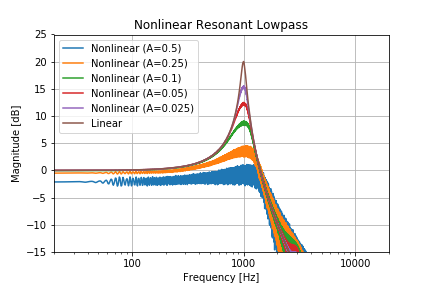
\includegraphics[width=3in]{../Pics/NL-LPF.png}
    \caption{\label{NL-LPF-freq}{\it Frequency responses of nonlinear biquad lowpass
                                    filters at varying amplitudes.}}
\end{figure}
%

\subsection{Digital Nonlinear Biquad}

We first construct this filter using the nonlinear biquad structure.
In \cref{NL-LPF-freq} we show the response of this filter for sine sweeps of
various amplitudes, compared to the frequency response of the corresponding
linear filter. In \cref{pzPlots} we show the movement of the poles and zeros of
the filter for varying steady state inputs. We calculate the instantaneous
poles using \cref{eq:poles_nl}, using $g_1 = g_2 = g$, as described in
each figure.
%
\begin{figure}[ht]
    \center
    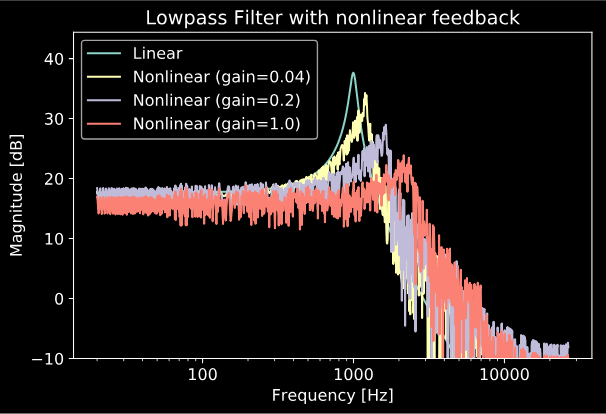
\includegraphics[width=3in]{../../NonlinearFeedback/Pics/LPF-NL.png}
    \caption{\label{NL2-LPF-freq}{\it Frequency responses of lowpass
                                    filters with nonlinear feedback
                                    at varying amplitudes.}}
\end{figure}
%

\subsection{Digital Nonlinear Feedback Filter}
%
Next, we construct the same resonant lowpass filter
using the nonlinear feedback structure. In \cref{NL2-LPF-freq},
we show the frequency response of the filter for sine sweeps of
various amplitudes. In \cref{pzPlots2} we show the movement of the
poles and zeros of the filter for various steady state gains. The
instantaneous poles are calculated using \cref{eq:poles_nl2}, again
using $g_1 = g_2 = g$.

\subsection{Using the Nonlinear Biquad for Analog Modelling}
%
To show how the nonlinear biquad filter structure can be useful
for analog modelling purposes, first note that the input gain to
the nonlinear biquad can be used as a tunable parameter (see \cref{50hz}).
\newline\newline
%
\begin{figure}[h]
    \center
    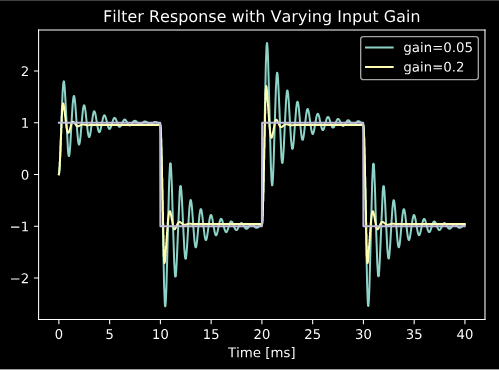
\includegraphics[width=3in]{../Pics/50-Hz_Response.png}
    \caption{\label{50hz}{\it Response of the nonlinear resonant lowpass
                            filter to a 50 Hz square wave with varying input gain.}}
\end{figure}
%
By tuning the input gain, we can attempt to match the response of an
arbitrary analog filter, either by tuning the parameters by ear
or using some form of numerical optimisation. Note that the choice
of base nonlinearities used by the nonlinear biquad will also play a
role in the accuracy of the model. For example, if the output of the
analog filter being modelled is asymmetric, then to accurately model
that filter, the nonlinear biquad must be constructed using an
asymmetric base nonlinearities.
%

\subsubsection{Comparison with Analog Filter}

As an example, we can attempt to construct a naive model of Sallen-Key
lowpass filter, a commonly used analog filter structure, and compare
with our results to the desired analog response similar to the
comparison done in \cite{SKF}. We describe this
as a naive model because we do not make any attempt to understand the physical
properties of the analog filter when constructing this model. We construct
a nonlinear biquad filter using $\tanh$ base nonlinearities, and design a
resonant lowpass filter with cutoff frequency $f_c = 1 \text{ kHz}$,
and $Q=10$, as well as a simulation of the corresponding Sallen-Key
filter using LTSpice. To accentuate the nonlinear behavior of the analog
filter, we choose $\pm 4 \text{ V}$ as the source voltages for the analog
filter circuit. We then compare the outputs of the two filters
for square waves at different frequencies, and use a simple staircase
optimisation scheme to find the input gain for the nonlinear biquad
that best matches the analog simulation. The results for the $250 \text{ Hz}$
square wave can be seen in \cref{SPICE}. While nonlinear biquad model
is not perfect, it does capture the damping effects of the analog filter
much more accurately than the corresponding linear filter, and can be greatly
improved with a more well-informed choice of base nonlinear functions, and
a more sophisticated optimisation scheme.
%
\begin{figure}[ht]
    \center
    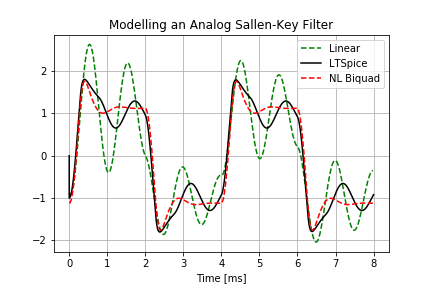
\includegraphics[width=3in]{../Pics/Spice-Compare.png}
    \caption{\label{SPICE}{\it Comparison between a linear resonant lowpass
                            filter, a resonant lowpass made with a nonlinear biquad
                            using a $\tanh$ clipper with input gain $0.283$,
                            and a SPICE simulation of a Sallen-Key lowpass.
                            All of the lowpass filters have $f_c=1$ kHz, and
                            $Q=10$. The input signal in each case is a $250$ Hz
                            square wave.}}
\end{figure}
%

\section{Conclusion}

In this paper, we have developed two structures for stable nonlinear biquad
filters. We have introduced the new architecture as a modification of the
Transposed Direct Form II filter form, and shown
how the changed architecture affects the pole locations depending on
the amplitude of the input signal. We have also derived constraints under
which the structure is guaranteed stable.
\newline\newline
As an example of the nonlinear biquad filter structure we have implemented
a resonant lowpass filter using both structures, and shown that the
poles respond to the input as expected. We then show how the nonlinear
biquad structure can be used to model an analog filter,
and comparing with a Sallen-Key lowpass filter as an example. Note
that while the nonlinear biquad structure can be used for analog modelling
both structures can also be used purely in the digital domain, as a tool
for constructing filters that sound more sonically interesting
and harmonically rich.
\newline\newline
To demonstrate this last point, we have also developed an open-source
audio plugin (VST, AU) implentation of the both nonlinear biquad and
nonlinear feedback filters, extending to several filter shapes, and
several base nonlinearities.
The source code for the plugin implementation is available on
GitHub\footnote{\url{https://github.com/jatinchowdhury18/ComplexNonlinearities}}.
\newline\newline
Future research concerning nonlinear filtering will center around making a
more informed choice of base nonlinearities, focusing on both the desired
harmonic response of the filter, as well as physically meaningful base
nonlinearities for use in analog modelling. Additionally, we would like
to investigate possible conditions under which the monotonicity
constraint from \cref{eq:NL_constraint} can be relaxed, allowing for
non-monotonic base nonlinearities such as wavefolders.

%\newpage
\nocite{*}
\bibliographystyle{IEEEbib}
\bibliography{references}

\end{document}
